\documentclass[11pt]{beamer}
\usetheme{Goettingen}
\usepackage[utf8]{inputenc}
\usepackage{amsmath}
\usepackage{amsfonts}
\usepackage{amssymb}
\usepackage{graphicx}
\usepackage{hyperref}
\author{Alex Heilman}
\title{Computational Cluster}
\subtitle{Basic Usage with Slurm}
%\setbeamercovered{transparent} 
%\setbeamertemplate{navigation symbols}{} 
%\logo{} 
%\institute{} 
%\date{} 
%\subject{} 


\addtobeamertemplate{navigation symbols}{}{%
	\usebeamerfont{footline}%
	\usebeamercolor[fg]{footline}%
	\hspace{1em}%
	\insertframenumber/\inserttotalframenumber
}


%Global Background must be put in preamble


\usepackage[style=numeric,backend=bibtex,sorting=none]{biblatex}

\addbibresource{chgcnn.bib}
\addbibresource{chgcnn.bib}


\newenvironment{boxed2}
    {\begin{center}
    \begin{tabular}{|p{0.95\textwidth}|}
    \hline\\
    }
    { 
    \\\\\hline
    \end{tabular} 
    \end{center}
    }


\begin{document}
	
	\begin{frame}
		\maketitle
	\end{frame}
	
	\begin{frame}{Overview}
	$\bullet$ Network architecture \& access
		
	\vspace{0.8cm}
		
	$\bullet$ Running commands across multiple machines with Ansible
			
	\vspace{0.8cm}
	
	$\bullet$ Slurm usage \& troubleshooting
	\end{frame}
	
	\begin{frame}[fragile=singleslide]\frametitle{Architecture}
	\begin{center}
		
	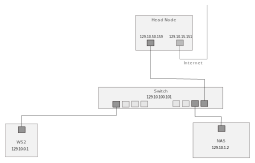
\includegraphics[scale=0.38]{qyg-c1-schem.pdf}
			
	All devices are on subnet of the gateway \verb|HeadNode|
	
	\end{center}
	\end{frame}
	
	\begin{frame}{What's a subnet?}
	$\bullet$ A subnet is assigned a subnet mask
	
	\vspace{0.5cm}
	
    $\bullet$ All IPs under it's mask are on the subnet
    	
    \vspace{0.5cm}
    
    $\bullet$ Subnet masks are specified by the gateway's IP address, ours is 255.255.0.0 or 129.10.0.0/16
	
	\vspace{0.5cm}
	
	$\bullet$ This means all nodes must have IP in range 129.10.x.x
	
	\end{frame}
			
	\begin{frame}[fragile=singleslide]\frametitle{What's a gateway?}
	$\bullet$ A gateway gives a LAN access to the larger internet.

	\vspace{0.5cm}	
	
	$\bullet$ The head node is configured with \verb|iptables|
	
	\vspace{0.5cm}
	
	$\bullet$ For new nodes, pass this command locally to set the default gateway:
	\begin{verbatim}
		sudo route add default gw 129.10.50.159
	\end{verbatim}
	\end{frame}
	
	\begin{frame}[fragile=singleslide]\frametitle{How to Access the Cluster}
		The worker nodes are on the subnet 129.10.X.X with the gateway set as 129.10.15.189 (the head node). 
		
		\vspace{0.8cm}
		
		$\bullet$ To access these nodes, use the -J option with SSH to jump through the head node.
		\begin{verbatim}
ssh -J <user>@129.10.15.189 <user>@<subnode-IP>
		\end{verbatim}

		$\bullet$ Append rule to ``$\sim$/.ssh/config" file to automatically jump with ProxyJump
		
	\end{frame}
		
	\begin{frame}[fragile=singleslide]\frametitle{What's a DNS server?}
	$\bullet$ A Domain Name Service (DNS) provides maps from IP to web addresses.
	
		
	\vspace{0.5cm}
	
	$\bullet$ DNS server is often set dynamically by network admins, we need to specify ourselves for subnodes.
	
	\vspace{0.5cm}
	
	$\bullet$ We can use Google's public DNS 8.8.8.8
	
	\vspace{0.5cm}
	
	$\bullet$ If broken, for quick fix:
	{\footnotesize
	\begin{verbatim}
echo "nameserver 8.8.8.8" | sudo tee /etc/resolv.conf > /dev/null
	\end{verbatim}}
	
	\end{frame}
	
	\begin{frame}[fragile=singleslide]\frametitle{Mounting the NAS}
	$\bullet$ We mount with NFS
	
	\vspace{0.45cm}
	
	$\bullet$ Must install \verb|nfs-common| on all devices
	
	\vspace{0.45cm}
	
	$\bullet$ Add line to \verb|/etc/fstab|:
	{\tiny
	\begin{verbatim}
		<NAS-IP>:/<NAS-Shared-Folder>   <Directory-to-Mount-to>    nfs    defaults    0 0 :
	\end{verbatim}}
	
	
	$\bullet$ Confirm \verb|/etc/fstab| isn't broken with \verb|findmnt --verify| 
	
	\vspace{0.45cm}
	
	$\bullet$ Reload \verb|/etc/fstab| with \verb|mount -a|
		
	\end{frame}
	
	
	\begin{frame}{What's Ansible?}
		
		Ansible allows us to run commands across several machines
		
		\begin{center}
			\includegraphics[scale=0.3]{screens/Ansible_logo.png}
		\end{center}
		
		\vspace{0.5cm}
		
		$\bullet$ State vs. action
		
		\vspace{0.3cm}
		
		$\bullet$ Idempotency
	\end{frame}
	
	\begin{frame}[fragile=singleslide]\frametitle{Defining Inventory/Ansible Hosts}
		$\bullet$ Must define host and group names of devices to run ansible commands
		
		\vspace{0.3cm}
		
		$\bullet$ These are specified in local inventory files or globally via \verb|/etc/ansible/hosts|
		
		\vspace{0.4cm}
		
		\begin{center}
			\includegraphics[scale=0.6]{screens/ansible_hosts.png}
		\end{center}
		The current hosts file is shown above.
	\end{frame}
	
	\begin{frame}[fragile=singleslide]\frametitle{Host Prerequisites}
		$\bullet$ Before running ansible, all hosts must be accesible by SSH without prompts.
		
		\vspace{0.5cm}
		
		$\bullet$ Generate RSA key pairs with command on head node:
		
		\begin{verbatim}
			ssh-keygen -t rsa
		\end{verbatim}
		
		$\ \ $ Then copy SSH keys to subnodes with:
		
		\begin{verbatim}
			ssh-copy-id <user>@<subnode-identifier>
		\end{verbatim}
		
		$\ \ $ After this, no password should be required.
	\end{frame}
	
	\begin{frame}[fragile=singleslide]\frametitle{Ex: Installing packages cluster-wide}
		$\bullet$ We can use ansible to install packages across all devices:
		
		\vspace{-0.21cm}
		
		\begin{verbatim}
			---
			- hosts: all
			tasks:
			- name: Install packages 
			apt:
			state: present
			name:
			- ntp
			- htop
			- vim
		\end{verbatim}
		
		\vspace{-0.55cm}
		
		We can run the above 'site.yml' playbook with:
		
		\vspace{-0.18cm}
		
		\begin{verbatim}
			ansible-playbook --ask-become-pass site.yml
		\end{verbatim}
		
		\vspace{-0.55cm}
		
		where the flag \verb|--ask-become-pass| will prompt for sudo password of current user.
	\end{frame}	
	
	\begin{frame}[fragile=singleslide]\frametitle{Ex: Setting up environments cluster-wide}
		$\bullet$ We can also use ansible to set up pip environments:
		
		\vspace{-0.18cm}
		
		\begin{verbatim}
			- name: install python packages with pip
			become: yes
			pip:
			name:
			- wheel
			- flask
			- gunicorn
			virtualenv: '/myproject/myprojectenv'
		\end{verbatim}
	\end{frame}	
	
	
	\begin{frame}{What's a daemon?}
	Daemons run in the background and process requests to services that run continuously, waiting for input
	
	\vspace{0.5cm}
	
	\begin{center}
		\includegraphics[scale=0.6]{screens/slurmctld_status.png}
	\end{center}

	
	
	\end{frame}
	
	\begin{frame}[fragile=singleslide]\frametitle{Systemctl}
	$\bullet$ System daemon controls other daemons through it's own: systemd.
	
	\vspace{0.6cm}
	
	$\bullet$ Start, stop, and enable services via systemctl
	
	\vspace{0.6cm}
	
	$\bullet$ On reboot, slurm daemons must be reset manually with 
	\begin{verbatim}
	systemctl start <daemon-name>
	scontrol update NodeName=<node-name> state=resume
	\end{verbatim}
	\end{frame}
		
	\begin{frame}[fragile=singleslide]\frametitle{What's Slurm?}	
	Slurm allows us to schedule jobs across the cluster
		
	\begin{center}
	\includegraphics[scale=0.3]{screens/Slurm_logo.png}
	\end{center}

	\vspace{0.6cm}
	
	$\bullet$ Head node runs \verb|slurmctld| daemon
	
	\vspace{0.3cm}

	$\bullet$ Worker nodes runs \verb|slurmd| daemon
	
	\vspace{0.6cm}
	\end{frame}
	
%	\begin{frame}{Slurm Prerequisites}
%	Munge, ntp, UIDs, slurm user + GIDs
%	\end{frame}
	
%	\begin{frame}{Installing Slurm}
%	download, configure, make, make install, create directories and change permissions, create and copy configuration, copy daemons, reload daemons, start and enable daemons
%	\end{frame}

\begin{frame}[fragile=singleslide]\frametitle{Using Slurm}
	$\bullet$ Logs are located at \verb|\var\log\<daemon-name>.log|

\vspace{0.5cm}

$\bullet$ Configuration file at \verb|\etc\slurm\slurm.conf|

\vspace{0.5cm}

$\bullet$ Try locating scripts and data needed to run in \verb|/mnt/nas|

\vspace{0.5cm}
\end{frame}

\begin{frame}[fragile=singleslide]\frametitle{Using Slurm}

$\bullet$ Check cluster status with \verb|sinfo|

		
\begin{center}
	\includegraphics[scale=0.55]{screens/sinfo.png}
\end{center}

$\bullet$ Check specific node with \verb|scontrol show node <name>|

		
\begin{center}
	\includegraphics[scale=0.55]{screens/scontrol_show.png}
\end{center}

\vspace{0.5cm}
\end{frame}
	
	\begin{frame}[fragile=singleslide]\frametitle{Using Slurm}

	
	$\bullet$ Run command on cluster with \verb|srun <command>|
	
	\vspace{0.5cm}
	
	$\bullet$ Submit script to scheduler with \verb|sbatch <script>|
	
	\vspace{0.5cm}
	
	$\bullet$ Check queue of jobs with \verb|squeue|
	
	\vspace{0.5cm}
	
	$\bullet$ Cancel job or allocation with \verb|scancel <job-id>|
	\end{frame}
	
	\begin{frame}[fragile=singleslide]\frametitle{Recap}
	$\bullet$ Network architecture \& access
	\begin{itemize}
		\item Need to jump through head node (gateway)!
		\item DNS server may be reset occasionally by restart
		\item NAS is mounted globally to \verb|\mnt\nas|
	\end{itemize}
	
	\vspace{0.3cm}
	
	$\bullet$ Can use Ansible for cluster-wide commands
	\begin{itemize}
		\item Install packages
		\item Create environments
		\item Setup Slurm
	\end{itemize}
	
	\vspace{0.3cm}
	
	$\bullet$ Schedule large jobs with Slurm
	\begin{itemize}
	\item Try to run from \verb|\mnt\nas|
	\item Check status of cluster with \verb|sinfo|
	\item Check status of jobs with \verb|squeue|
	\item Use \verb|sbatch| for scripts and \verb|srun| for commands
	\end{itemize}
	
	\end{frame}
	
	\begin{frame}[fragile=singleslide]\frametitle{Recap}
	
	$\bullet$ Problems?
	\begin{itemize}
	\item Confirm \verb|$PATH| contains Slurm \verb|bin| directory
	\item Check node with \verb|scontrol show node|
	\item Check daemons with \verb|systemctl status|
	\item Check logs at \verb|\var\log|
	\item Maybe contact me
	\end{itemize}

		
	\end{frame}



\end{document}